\chapter[What if we would use a diagnostic multi-cancer gene panel for opportunistic screening? A study in 2,090 Dutch familial cancer patients]{What if we would use a diagnostic multi-cancer gene panel for opportunistic screening? A study in 2,090 Dutch familial cancer patients}
\chaptermark{opportunistic screening in familial cancer}
\label{chap:Opportunistic_screening}

{ \Large \leftwatermark{
		\put(-67,-66.5){ 1 }
		\put(-67,-91.5){ 2 }
		\put(-67,-116.5){ 3 }
		\put(-76.5,-150){
\includegraphics[scale=0.8]{img/thumbindex.eps}} \put(-67,-141.5){ {\color{white} 4 }}
		\put(-67,-166.5){ 5 }
		\put(-67,-191.5){ 6 }
		\put(-67,-216.5){ 7 }
		\put(-67,-241.5){ 8 }
		\put(-67,-266.5){ 9 }
		\put(-67,-291.5){ 10 }
		\put(-67,-316.5){ 11 }
	} \rightwatermark{
		\put(350.5,-66.5){ 1 }
		\put(350.5,-91.5){ 2 }
		\put(350.5,-116.5){ 3 }
		\put(346.5,-150){
\includegraphics[scale=0.8]{img/thumbindex.eps}} \put(350.5,-141.5){ {\color{white} 4 }}
		\put(350.5,-166.5){ 5 }
		\put(350.5,-191.5){ 6 }
		\put(350.5,-216.5){ 7 }
		\put(350.5,-241.5){ 8 }
		\put(350.5,-266.5){ 9 }
		\put(350.5,-291.5){ 10 }
		\put(350.5,-316.5){ 11 }
}}

\hfill \underline{submitted} 


\newpage

\noindent
L.F. Johansson\textsuperscript{1}, K.K. van Dijk-Bos\textsuperscript{1}, A.H. van der Hout\textsuperscript{1}, A.P. Knopperts\textsuperscript{1}, B. Leegte\textsuperscript{1}, P.C. van den Akker\textsuperscript{1}, K. Kok\textsuperscript{1}, I.M. van Langen\textsuperscript{1}, M.A. Swertz\textsuperscript{1}, R.K. Weersma\textsuperscript{2}, R.J. Sinke\textsuperscript{1}, B. Sikkema-Raddatz\textsuperscript{1}, H. Westers\textsuperscript{1,*}, R.H. Sijmons\textsuperscript{1,*}\\


\noindent
University of Groningen, University Medical Center Groningen, 1. Department of Genetics, 2. Department of Gastroenterology, Groningen, The Netherlands\\

\noindent* these authors contributed equally to the paper


\section*{Abstract}\label{abstract}
\subsubsection{Purpose}
In familial cancer (FC) diagnostics, analysis of next-generation sequencing data typically focuses on genes known to be associated with the cancer type that prompted referral. Currently, however, it is debated whether opportunistic screening should be performed when sequence data is available for other genes. We aimed to determine how many secondary findings (SFs) would be detected in cancer-predisposing genes present in our FC gene panel if we offered opportunistic screening to patients within FC diagnostics.
\subsubsection{Methods}
We anonymously reanalyzed sequencing data of 2,090 FC patients for either 73 genes (original FC panel) or 85 genes (updated panel) for SNVs, indels and CNVs. To determine the background prevalence of pathogenic variants in FC genes, we screened 1,326 individuals from the general Dutch population.
\subsubsection{Results}
We detected SFs in 3.0\% of patients (excluding heterozygous CHEK2 and MUTYH variants), and a (likely) pathogenic variant matching their family’s cancer type in 10.1\% of patients. In the Dutch population cohort, 3.2\% of individuals had a (likely) pathogenic variant in a cancer-predisposing gene. 
\subsubsection{Conclusion}
Our results can assist in the design of future research programs on opportunistic screening. These programs are needed because there is not yet sufficient evidence to meet international screening program criteria. 

\section{Introduction}\label{introduction}
Next-generation sequencing (NGS) allows for simultaneous diagnostic testing of many genes, and NGS gene panels are now commonly used in familial cancer (FC) diagnostics \cite{Okur_2017}. 
These panels typically target particular tumor types or a combination of them (e.g. colorectal cancer or breast and ovarian cancer). 
This approach deliberately limits the chance of detecting pathogenic variants in genes associated with cancer types other than the tumor types that triggered referral, i.e. secondary findings (SFs) \cite{DeRycke_2017,Concolino_2018}. 
Diagnostic panels could, however, be used for other purposes. 
Firstly, the systematic use in FC diagnostics of broader gene panels, including new candidate cancer-predisposing genes, could help define the phenotypes associated with variants in newly postulated genes. 
This might, in time, increase the molecular diagnostic yield in patients referred for FC, as ~90\% of these patients are currently left without a molecular diagnosis \cite{Tung_2016,Thompson_2016,Minion_2015,LaDuca_2014}. 
Secondly, extended panels would allow for opportunistic screening for actionable variants in a broader range of cancer-predisposing genes, rather than limiting their use to the genes associated with the cancer type(s) that prompted referral. The pros and cons of opportunistic genetic screening and reporting SFs in patients who undergo diagnostic testing are currently the subject of a debate triggered by statements by the American College of Medical Genetics and Genomics (ACMG) that advocate such screening and reporting \cite{Green_2013,Burke_2013,Yu_2014,Kalia_2016,Haer_Wigman_2018,Wouters_2018,Brothers_2019,Esplin_2018}. 
Performing this kind of screening in addition to diagnostics is not part of current Dutch clinical genetics services because it would be regarded as population screening, which is not allowed without special permission by Dutch authorities. However, screening could be of health benefit to our patients, and therefore further discussion is thus warranted in the context of a clinical genetics service system that is already under pressure by increasing numbers of referrals. 
As part of this discussion, it is important to establish the scope and frequency of SFs we expect to see if broad diagnostic cancer gene panels are used for screening. 

We developed an 85-gene, multi-cancer targeted NGS gene panel and implemented it in our genome diagnostics laboratory. 
For diagnostic purposes clinicians in our center can request analysis of only particular subsets of genes in the panel that are known to be related to the tumor types in families. 
For research purposes, all panel genes, including newly postulated tumor syndrome genes, are analyzed anonymously for all patients.

The primary aim of this study was to estimate the number of SFs that we would detect if, in addition to diagnostic testing, we were to screen for variants in genes beyond those with known associations to the referral cancer type. 
We sought to estimate this number against the background of diagnostic yield of our gene panel in a cohort of 2,090 patients referred to our clinic for FC diagnostics, a process that included the testing for single nucleotide variants (SNV), indel variants and copy number variants (CNV). 
In the near future opportunistic screening for cancer-related variants, and others that are outside the scope of our paper, could be made available to more patients as exome testing becomes more prevalent for many types of conditions. 
To estimate the number of SFs in case of opportunistic screening in Dutch patients, in general, we also analyzed SNVs, indels and CNVs in the 85 panel genes in the dataset of all 498 non-related individuals from the Dutch genome sequencing project Genome of the Netherlands (GoNL) \cite{Francioli_2014} and in exome data of 828 samples from the LifeLines Deep (LLD) consortium, which is representative of the population in the northern Netherlands \cite{Tigchelaar_2015}.
Another reason for the population study was that if we would find significantly more SFs in our FC cohort than expected given general population frequencies, this would suggest that some of the SFs might actually be diagnostic, reflecting expanded tumor syndrome phenotypes.

Across these analyses, we determined which variants would be eligible for return based on two sets of guidelines that list genes eligible for return of SFs: one recommended by the ACMG and one from the French Society of Predictive and Personalized Medicine (SFMPP). 
Based on our results, we assessed if such screening meets proposed genetic screening criteria \cite{Andermann_2008}. 
Hereby we aim to add context to the discussion if, or which, variants should be returned to an individual in absence of a reason for diagnostic testing for those variants. 

\section{Materials and Methods}\label{methods}
\subsection{Patient cohorts}
This study was performed in accordance with Dutch and University Medical Center Groningen (UMCG) ethical guidelines. 
All patients involved had been referred to the FC Clinic of the department of Genetics of the UMCG for genetic diagnostics and counseling. 
Patients were seen between March 2013 and January 2017. Referrals for testing met the Dutch guidelines for genetic testing \cite{Erfelijk_2010}. 
For molecular diagnostic purposes, only those genes from the NGS panel that were in the differential diagnosis for the patient and family tumor type, were analyzed. 
The outcomes of these “virtual” subpanels extracted from the full dataset were reported to the genetic counselor and discussed with the patient and referring physician. 
For the purpose of our research, the sequencing data of all panel genes were analyzed anonymously in all patients. 
Personal and family histories regarding tumors (including intestinal polyps) were available. 

Our patient population for FC panel testing consisted of two cohorts: \newline
\noindent\textbf{Cohort A (n=198)} is a ‘retrospective cohort’ of patients who previously tested negative, using Sanger sequencing, for selected genes that seemed most appropriate given their cancer type (e.g. \textsl{BRCA1/2} in breast cancer patients). 
These patients were sequenced using the NGS panel in 2013 and 2014 and were selected based on having the pedigrees most suspect for a genetic predisposition: their age at cancer diagnosis was at least 5 years younger than the minimum age in the referral guidelines and/or they had more than the minimum number of affected relatives required for referral. 
We included this cohort because it reflects our clinical practice of re-analyzing unsolved families, especially the more suspect ones, with new techniques.
\newline
\noindent\textbf{Cohort B (n=1,892)} is a ‘prospective cohort’ of patients referred to our clinical genetics department between 2014 and 2017 for FC diagnostics. 
Subpanel testing was the first genetic diagnostic test performed in these patients. 

\subsection{General Dutch population cohort}
We used data from two general Dutch population cohorts to determine the population frequency of variants in the genes in our targeted panel. 
The first cohort is a representative subset of the Dutch population produced by the GoNL project, from which we included 498 non-related individuals \cite{Francioli_2014}. 
The second cohort consists of 828 participants of the LLD cohort \cite{Tigchelaar_2015}. 
Possible cancer phenotypes of GoNL or LLD participants were unknown to the researchers and cannot be excluded. Further details are available in the supplementary methods.

\subsection{Selection of genes for the NGS panel}
In March 2013, as part of our clinical FC diagnostics service in the UMCG, we developed and validated an NGS panel that contained 73 tumor syndrome genes (SureSelectXT Custom design \#0421101, referred to as panel 1 here) (Agilent Technologies, Santa Clara, CA). 
The design and validation methods for this panel have been reported previously \cite{Sikkema_Raddatz_2013}. 
In June 2015, the panel was updated with the addition of 13 genes and the removal of one gene, resulting in an 85-gene panel (SureSelectXT Custom design \#0735701, referred to as panel 2 here) (table \ref{table:screening_table1}).
The Fanconi anemia genes (other than \textsl{BRCA2} and \textsl{PALB2}) were left out of the panel as these were included in a separate hematology panel (not tested in our study). 

\begin{table}
\caption[Panel 1 and 2 genes and ACMG and SFMPP inclusion]{Genes present on panels 1 and 2 and their inclusion on the ACMG and SFMPP lists for recommended return.}
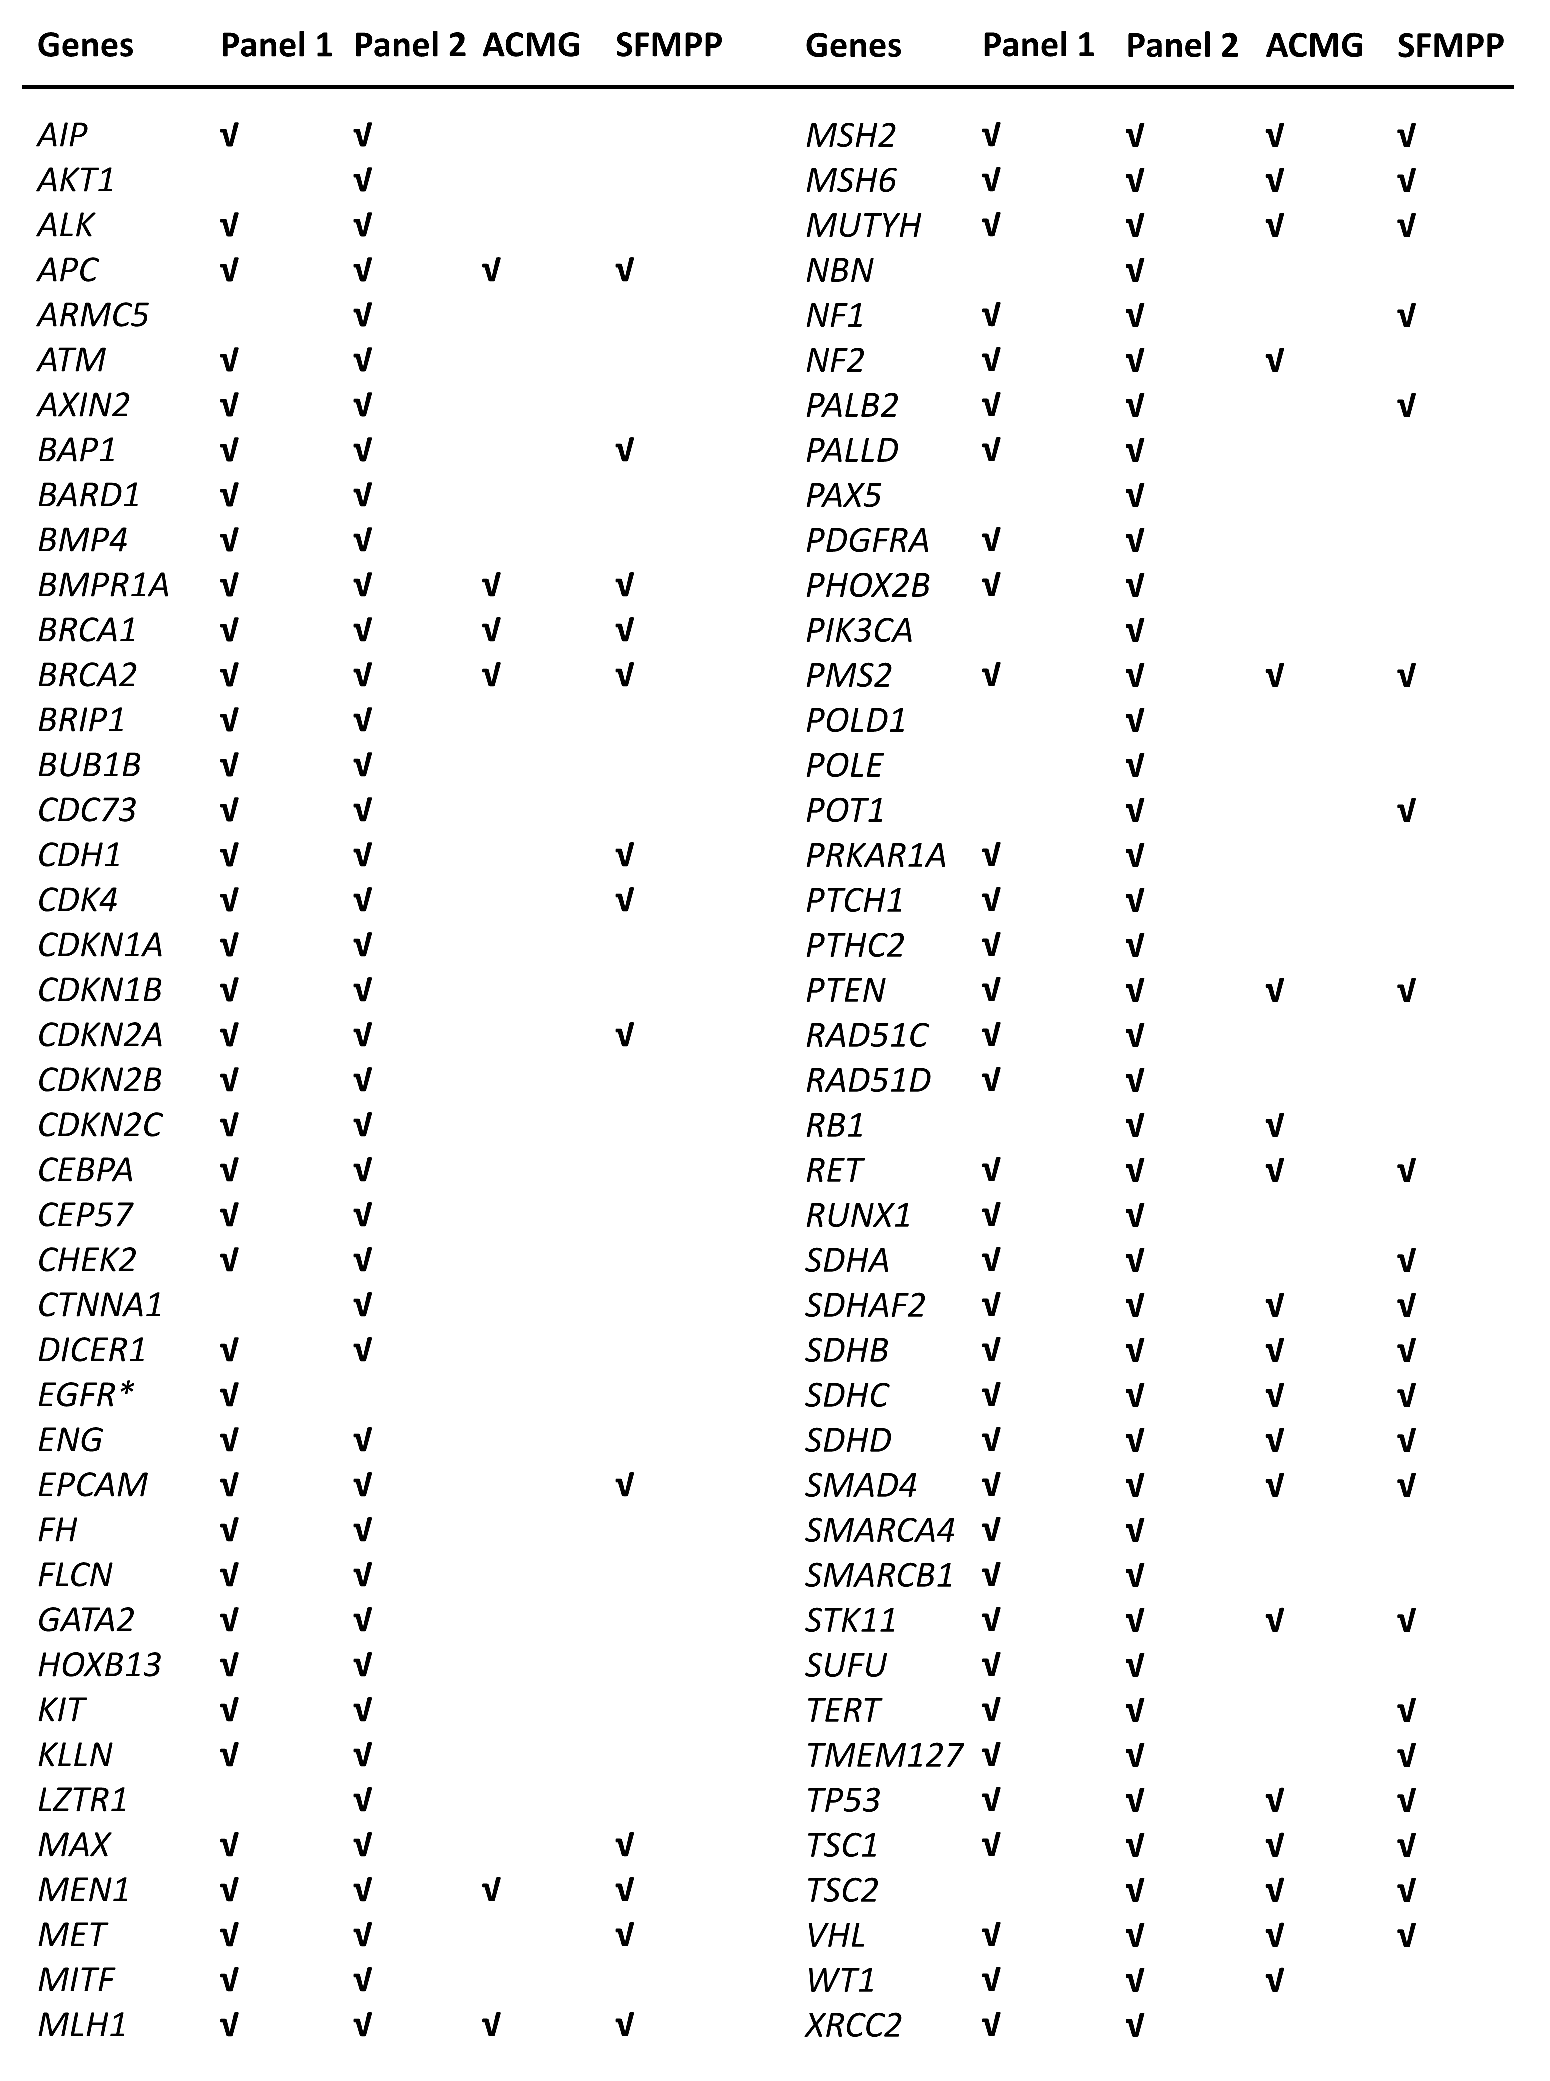
\includegraphics[width=1.0\linewidth]{img/opportunistic_screening_Table1}
 \caption*{\footnotesize{*not included in analysis}}
\label{table:screening_table1}
\end{table}

\subsection{Sequencing and alignment procedure}
All samples were prepared and sequenced according to the SureSelectXT Automated Target Enrichment for Illumina Paired-End Multiplexed Sequencing protocol (Agilent Technologies). 
In short, high molecular DNA was isolated from peripheral blood lymphocytes and randomly fragmented, followed by end repair, dA tailing and adapter ligation. 
Regions of interest were captured using a biotinylated cRNA probe solution (Agilent Technologies) using one of the two panels. Subsequently 151 bp paired-end sequencing was performed on an Illumina Miseq. 
Reads were aligned using Burrows-Wheeler Aligner (BWA) v0.7.12 \cite{Li_2010}. 
SNVs and indels were called using GATK HaplotypeCaller v3.5 and CNVs using CoNVaDING \cite{Johansson_2016b} and XHMM \cite{Fromer_2012}. 
Complete procedures are described in the supplementary methods. 
CNV calls of more than two exons that were made by both tools in samples that passed both CoNVaDING and XHMM sample quality control (QC) metrics were considered reliable and were not tested using another technique. 
All other calls were confirmed using either the Illumina HumanCytoSNP-850K-8 v1.1 array (Illumina, San Diego, CA) or the Multiplex Ligation-dependent Probe Amplification (MRC-Holland, Amsterdam, the Netherlands) using the manufacturer’s protocols. 

\subsection{Data analysis and interpretation}
The 198 patients in Cohort A (negative previous single gene analysis) and 299 patients from Cohort B were analyzed with gene panel 1. 
They were also screened for the \textsl{POLE} c.1270C$\textgreater$G (p.L424V) and POLD1 c.1433G$\textgreater$A (p.S478N) hotspot variants \cite{Palles_2012} using Sanger sequencing (as explained in the supplementary methods). 
The remaining 1,593 patients were analyzed using panel 2. 
For the general Dutch population samples only variants in our 85 panel genes were interpreted. 
No CNV detection was performed in the LLD samples.

The variant analysis we use in the UMCG clinical genetics department is based on the ACMG rules \cite{Richards_2015}. 
All annotated variants were analyzed using Cartagenia software (Agilent Technologies Bench Lab NGS v4.3.5) and Alamut (Alamut version 2.4, Interactive Biosoftware, Rouen, France). 
Variants were labeled in five classes (benign, likely benign, variant of unknown clinical significance (VUS), likely pathogenic and pathogenic) following the proposal of Plon et al \cite{Plon_2008}, with VUS equaling class III.

Variants were considered to add to the molecular diagnostic yield if they were labeled as pathogenic or likely pathogenic and found in a gene with an established relationship to (at least one of) the referral cancer type(s). This included both highly penetrant and more moderately penetrant variants (\textsl{e.g.} in \textsl{CHEK2)}. 
\textsl{MUTYH} variants were only included if they were homozygous or compound heterozygous. 
Variants were considered SFs when they were labeled (likely) pathogenic and had no established relation to any of the referral cancer types. 
Some SFs may actually turn out to represent extended phenotypes associated with the genes in question and thus go on to become primary findings. 
Some of these extensions have already been suggested, but not yet proven, in the literature. We therefore labelled SFs for which extended phenotypes have been suggested to match the patient’s referral cancer type as ‘suggested’. 
Variants in our analysis are thus labelled as having established, suggested or no relation with the referral cancer type(s). 
To determine how many actionable SFs would be found, (likely) pathogenic variants in the population cohorts were further filtered based upon two lists of genes in which (likely) pathogenic variants are considered to be actionable and recommended for return: the ACMG SF v2.0 list \cite{Kalia_2016}, which contains 25 cancer-related genes, all present in our panel, and 36 cancer-related genes from the SFMPP list \cite{Pujol_2018}, of which 35 are present in our panel (table \ref{table:screening_table1}).

All the variants detected in our study have been submitted to the public locus-specific databases of the Leiden Open Variant Database platform (www.lovd.nl/3.0/home). 

\section{Results}
\subsection{Sequencing quality}
For all samples, NGS quality met the criteria used in our genome diagnostic laboratory ($\textgreater$80\% of the bases were sequenced with a quality $\ge$Q30). 
After alignment and duplicate removal, the average coverage for targeted regions was 423$\times$ (sd 161$\times$) and 447$\times$ (sd 307$\times$) for panels 1 and 2, respectively, and \textgreater98\% of targeted bases were covered by at least 20 reads. 
Of the samples, 197 (99.5\%) retrospective cohort samples and 1,520 (95.4\%) prospective cohort samples passed CoNVaDING sample QC and were suitable for single exon CNV detection.     

\begin{table}
	\caption[Number of pathogenic variants found per referral cancer type]{\textbf{Number of pathogenic and likely pathogenic variants found per referral cancer type}}
	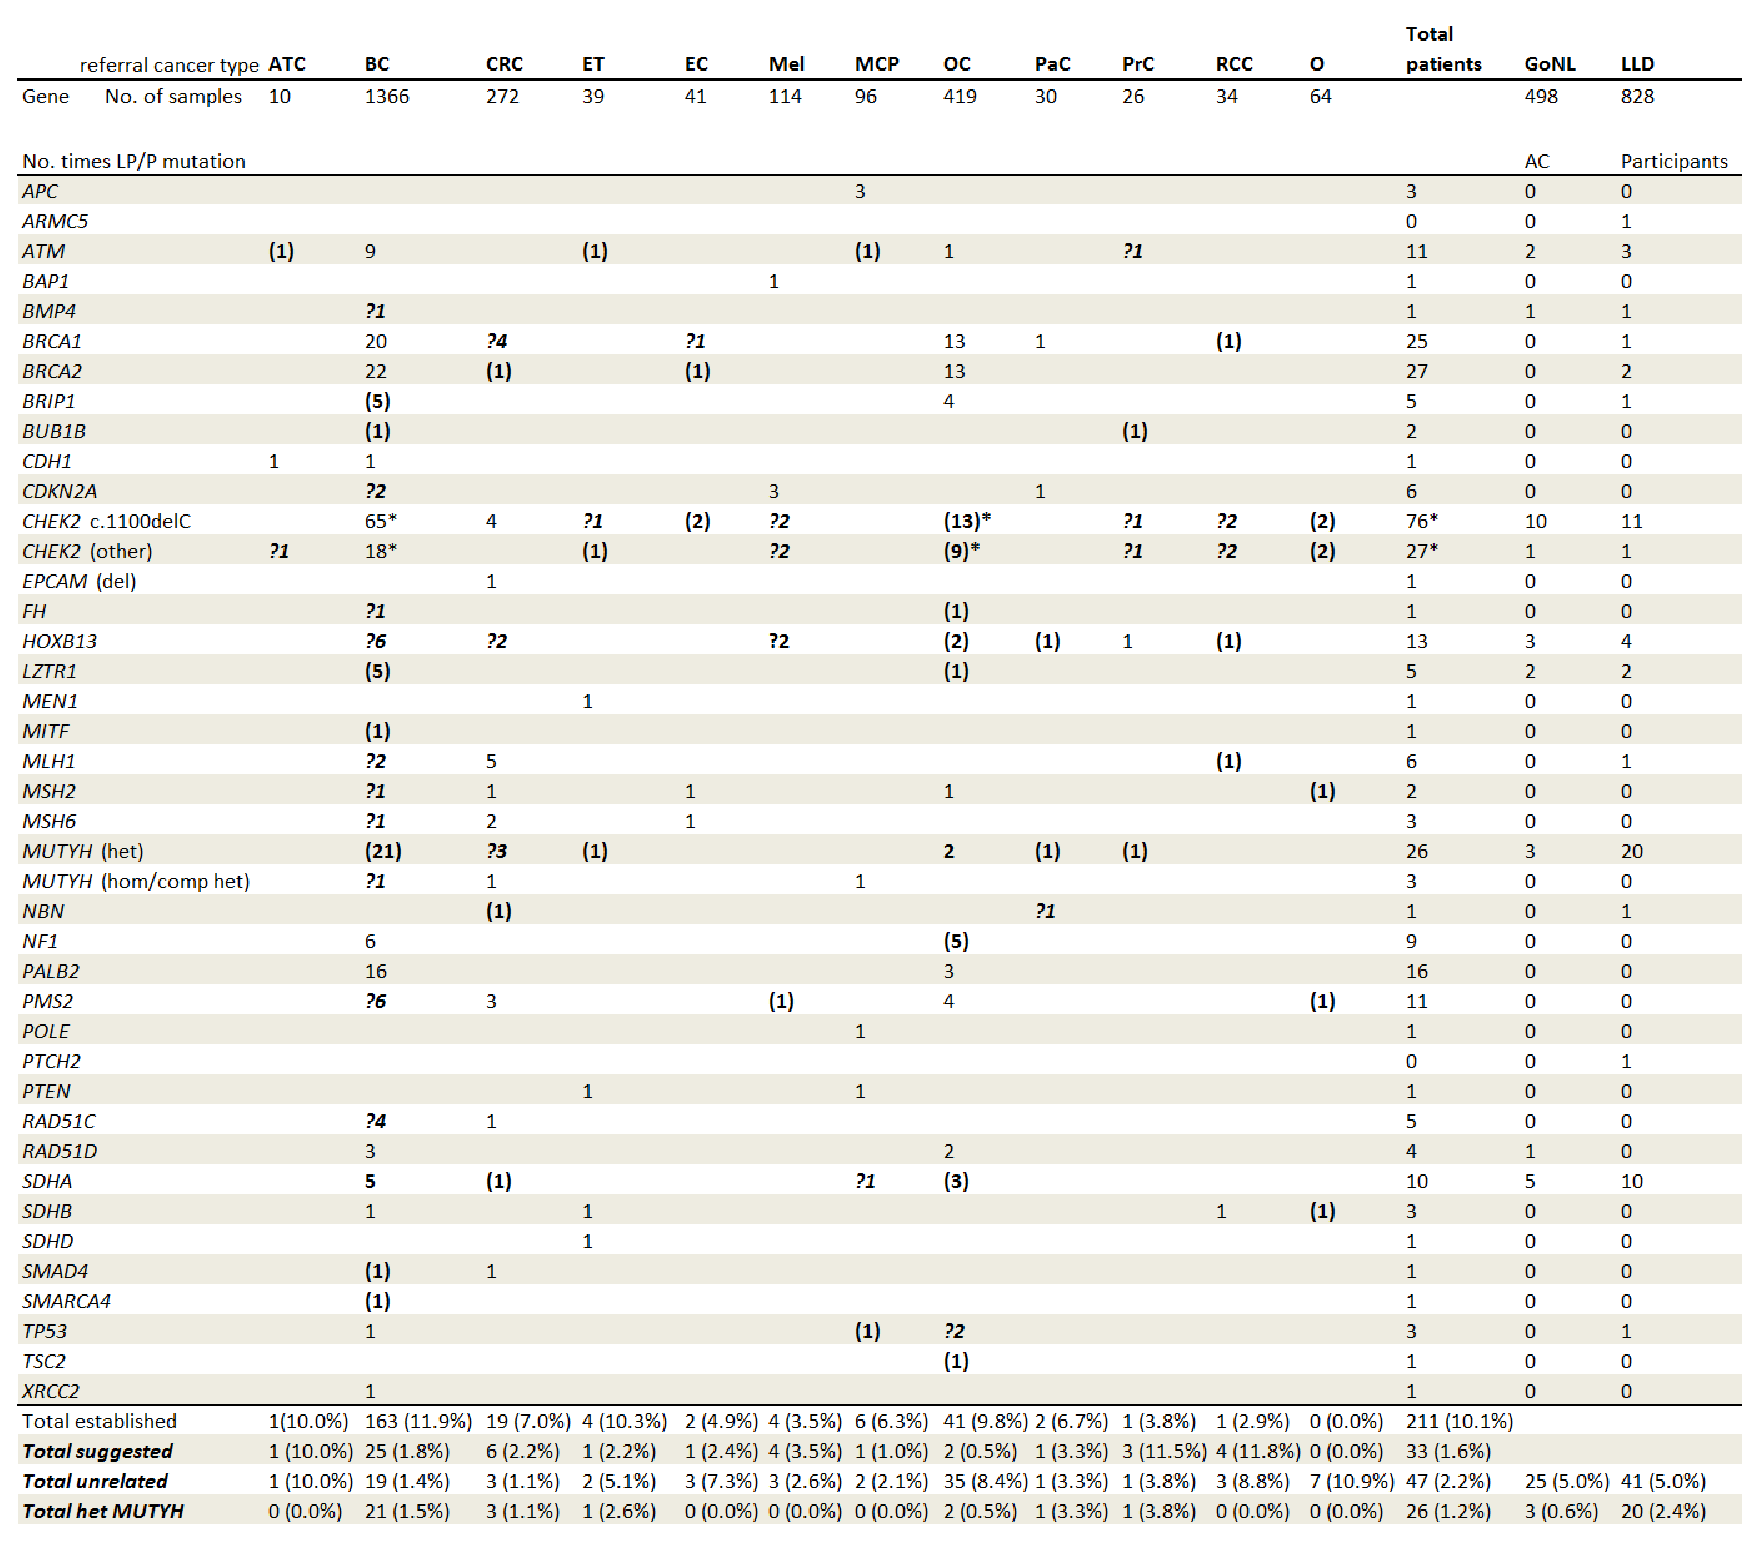
\includegraphics[width=1.0\linewidth]{img/opportunistic_screening_Table2}  %%Font does not support bold italic text.
		\caption*{\footnotesize{Plain text = gene with established relation to cancer phenotype; \textbf{Bold} text = secondary finding, encompassing: \textbf{Bold ()} = Gene with no relation to cancer phenotype; \begin{bfseries}\textit{Bold Italics ?}\end{bfseries} = Gene with suggested relation to cancer phenotype, *One sample homozygous or compound heterozygous, **All three positive instances have gastric cancer as the referral cancer type, ***Various endocrine tumor types (\textsl{ATM} and \textsl{CHEK2} other: neuroendocrine tumor; \textsl{CHEK2} c.1100delC, \textsl{MUTYH} het, \textsl{PTEN} and \textsl{SDHB}: Thyroid cancer; \textsl{MEN1}: Parathyroid adenoma; \textsl{SDHD}: Paraganglioma). ATC: alimentary tract cancer; BC: breast cancer; CRC: colorectal cancer; ET: endocrine tumor; EC: endometrial cancer; Mel: melanoma; MCP: multiple colorectal polyps; OC: ovarian cancer; PaC: pancreatic cancer; PrC: prostate cancer; RCC: renal cell cancer; O: Other cancer types; GoNL: Genome of the Netherlands cohort; LLD: Lifelines Deep cohort; AC: Allele count; het: heterozygous; hom: homozygous; ch: compound heterozygous. Genes without any likely pathogenic or pathogenic variant in any of the cohorts: \textsl{AIP}, \textsl{AKT1}, \textsl{ALK}, \textsl{AXIN2}, \textsl{BARD1}, \textsl{BMPR1A}, \textsl{CDC73}, \textsl{CDK4}, \textsl{CDKN1A}, \textsl{CDKN1B}, \textsl{CDKN2B}, \textsl{CDKN2C}, \textsl{CEBPA}, \textsl{CEP57}, \textsl{CTNNA1}, \textsl{DICER1}, \textsl{ENG}, \textsl{FLCN}, \textsl{GATA2}, \textsl{KIT}, \textsl{KLLN}, \textsl{MAX}, \textsl{MET}, \textsl{NF2}, \textsl{PALLD}, \textsl{PAX5}, \textsl{PDGFRA}, \textsl{PHOX2B}, \textsl{PIK3CA}, \textsl{POLD1}, \textsl{POT1}, \textsl{PRKAR1A}, \textsl{PTCH1}, \textsl{RB1}, \textsl{RET}, \textsl{RUNX1}, \textsl{SDHAF2}, \textsl{SDHC}, \textsl{SMARCB1}, \textsl{STK11}, \textsl{SUFU}, \textsl{TERT}, \textsl{TMEM127}, \textsl{TSC1}, \textsl{VHL}, \textsl{WT1}.}
	}
	\label{table:screening_table2}
\end{table}

\subsection{Patient cohort: variant analysis for diagnostic yield and secondary findings}
In the combined cohorts of 2,090 patients, we detected 324 pathogenic or likely pathogenic variants (SNV, indel and CNV) in 302 (14.4\%) patients distributed over 37 of the genes included in the panel, including two homozygous and three compound heterozygous variants (Table \ref{table:screening_table2} and Supplementary table 1). %%INSERT TABLE
In 48 genes no (likely) pathogenic variants were found.
In the retrospective cohort (n=198) we found 18 (likely) pathogenic variants in 16 patients (8.1\%). 
None of these were CNVs. 
Of the 18 (likely) pathogenic variants, 14 (7.1\%) had an established relation to at least one of the phenotypes warranting referral (Table \ref{table:screening_table3} \& Supplementary table 2). 

\begin{table}
	\caption[Genes with pathogenic and likely pathogenic variants]{\textbf{Genes with pathogenic and likely pathogenic variants}}
	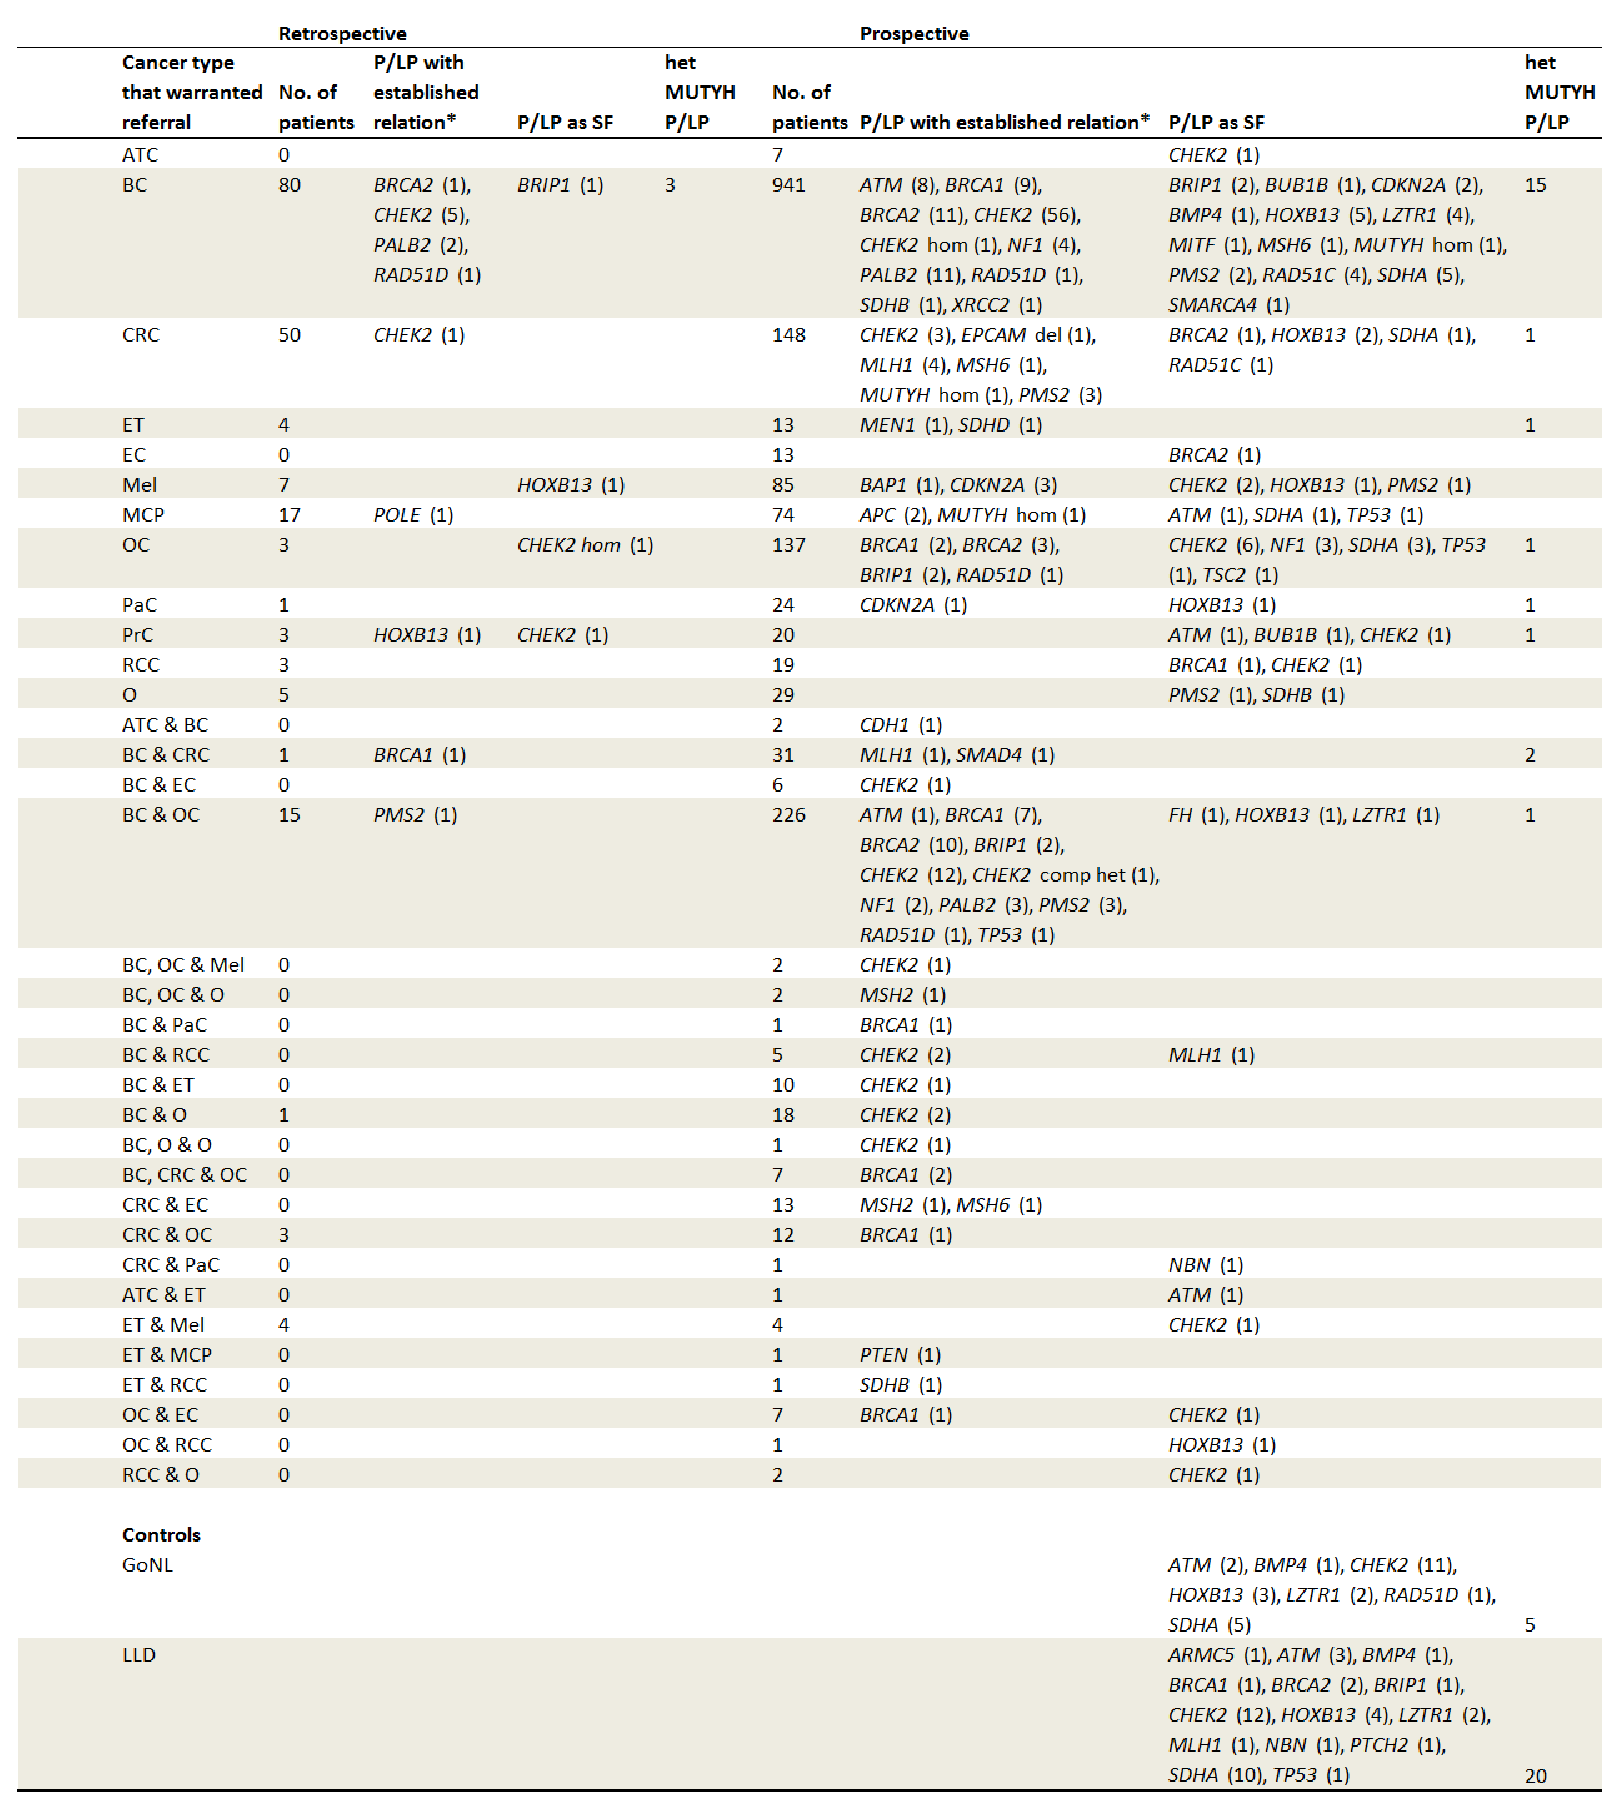
\includegraphics[width=1.0\linewidth]{img/opportunistic_screening_Table3}
		\caption*{\footnotesize{\textsl{Gene} (number of times (likely) pathogenic variant in gene); ATC: alimentary tract cancer; BC: breast cancer; CRC: colorectal cancer; ET: endocrine tumor; EC: endometrial cancer; Mel: melanoma; MCP: multiple colorectal polyps; OC: ovarian cancer; PaC: pancreatic cancer; PrC: prostate cancer; RCC: renal cell cancer; O: Other cancer types; GoNL: Genome of the Netherlands cohort; LLD: Lifelines Deep cohort. *to at least one of the cancer phenotypes}}
	\label{table:screening_table3}
\end{table}

The remaining four variants (2.0\%) were classified as SF. 
Two of these patients also had a pathogenic variant with an established relation to the referral cancer type (Table \ref{table:screening_table3} \& Supplementary table 3). 
Of the four SFs one was suggested to be related to the referral cancer type. 
Further research may confirm or disprove this suggestion. None of the four SFs were on the ACMG or SFMPP lists for recommended return. 
In addition, three heterozygous MUTYH pathogenic variants were found (Table \ref{table:screening_table3} \& Supplementary table 4). %insert table
A total of 54 VUSs were found (27.3\%), including four CNVs. 
In the prospective cohort (n=1,892), in 197 patients (10.4\%), we found a (likely) pathogenic variant in a gene that could explain or might have contributed to the family’s cancer type and that matched the patient’s reason for referral (Figure \ref{fig:screening_Fig1}, Table \ref{table:screening_table3} \& Supplementary table 2). %insert table and figure
Of these patients, two carried two independent (likely) pathogenic variants that matched their cancer type(s), and four carried a compound heterozygous or homozygous variant (2$\times$  \textsl{CHEK2} and 2$\times$  \textsl{MUTYH}). 
We excluded 23 heterozygous \textsl{MUTYH} variants (Table \ref{table:screening_table3} \& Supplementary table 4). %Insert table
Of the 201 (likely) pathogenic variants, 13 were CNVs. In addition, SFs were detected in 74 patients (3.9\%). 
Of these patients, two had two different SFs and eight had a second (likely) pathogenic variant with an established relation to the referral cancer type (Table \ref{table:screening_table3} \& Supplementary table 3). 
Of these 76 SFs, 32 have been suggested in the literature to be related to the referral cancer type. 
Further research may confirm or disprove these suggestions. The remaining 44 SFs had no established or suggested relation to any of the referral cancer types (2.3\% of patients when including heterozygous \textsl{CHEK2} variants and 2.0\% when excluding them). 
Of the 80 SFs found in the combined cohorts, including six CNVs, 14 (0.7\% of patients) would have been reported following ACMG recommendations (\textsl{MLH1}, \textsl{PMS2}, \textsl{BRCA1}, \textsl{BRCA2}, \textsl{MUTYH}, \textsl{PMS2}, \textsl{SDHB}, \textsl{TP53} and \textsl{TSC2}). 
When following the SFMPP list, an additional 15 SFs would have been reported (\textsl{CDKNA2}, \textsl{NF1} and \textsl{SDHA}), leading to a total of 1.4\% of patients. 
For the 80 SFs we found, 17 (21.3\% of SFs / 0.8\% of patients) have an established relation with other cancer types in the patient or family that were insufficient reason for genetic testing. 
In addition, 592 VUS were found, including 11 CNVs, in 492 patients in the prospective cohort.


\begin{figure}
	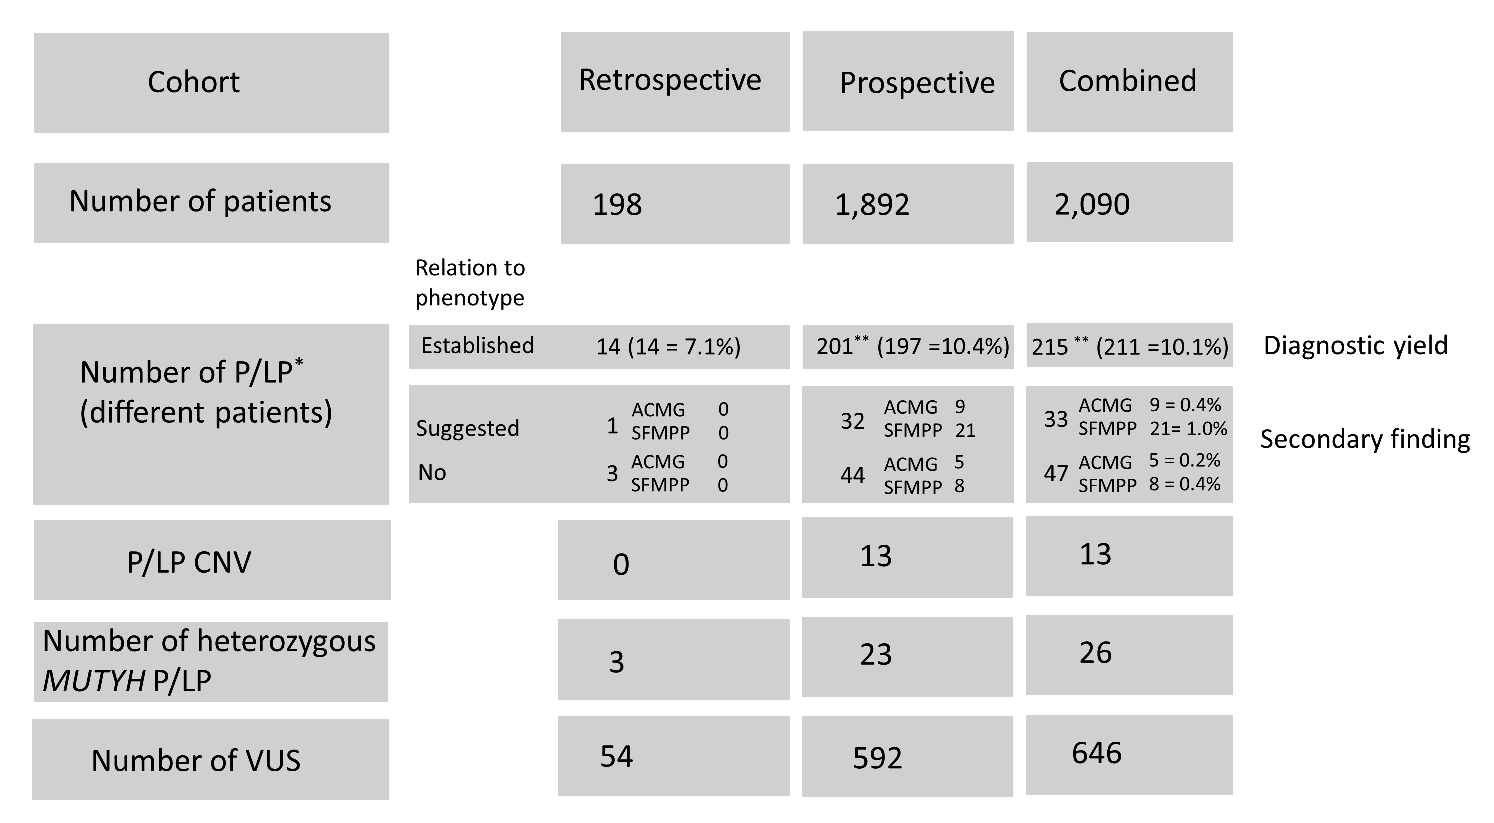
\includegraphics[width=1.0\linewidth]{img/opportunistic_screening_Fig1}
	\caption[Number of detected variants]{Number of detected variants in the retrospective and prospective cohorts with their relation to the referral cancer type. \footnotesize{*excluding heterozygous \textsl{MUTYH} variants. **compound heterozygous and homozygous variants both counted.}
	}
	\label{fig:screening_Fig1}
\end{figure}


The diagnostic yield percentages and SFs did not differ significantly between the retrospective and prospective cohorts (p-values Fisher’s Exact test (FET) \textgreater0.05).

\subsection{Control cohorts variant analysis}
To determine the expected yield of opportunistic screening in cancer-predisposing genes in patients referred for conditions other than FC we searched for (likely) pathogenic variants in the genes targeted by panel 2 in two control cohorts. 
In our cross-sectional Dutch population cohort of 498 individuals from the GoNL genome sequencing study, 14 (2.8\% when assuming a maximum of one pathogenic variant per individual) (likely) pathogenic variants were found in these genes (\textsl{ATM} 2$\times$, \textsl{BMP4}, \textsl{HOXB13} 3$\times$, \textsl{LZTR1} 2$\times$, \textsl{RAD51D}, \textsl{SDHA} 5$\times$), without including 11 (2.2\%) \textsl{CHEK2} and three (0.6\%) \textsl{MUTYH} variants (Table \ref{table:screening_table3} \& Supplementary table 5). %%INSERT TABLE
In addition, 106 VUS were found. Three of the \textsl{SDHA} variants concerned the same deletion of exons 6 and 7. 
None of the (likely) pathogenic variants were in genes present on the ACMG list for recommended return, while the five (1.0\%) \textsl{SDHA} variants are suggested to be reported by the SFMPP guidelines.

In the exome sequencing data of the 828 individuals from the LLD cohort, 29 (3.5\%) (likely) pathogenic variants were found in the genes targeted by panel 2 (\textsl{ARMC5}, \textsl{ATM} 3$\times$, \textsl{BMP4}, \textsl{BRCA1}, \textsl{BRCA2} 2$\times$, \textsl{BRIP1}, \textsl{HOXB13} 4$\times$, \textsl{LZTR1} 2$\times$, \textsl{MLH1}, \textsl{NBN}, \textsl{PTCH2}, \textsl{SDHA} 10$\times$, \textsl{TP53}), excluding 12 (1.5\%) heterozygous \textsl{CHEK2} and 20 (2.4\%) heterozygous \textsl{MUTYH} variants (Table \ref{table:screening_table3} \& Supplementary table 6).  %%INSERT TABLE
In addition, 172 VUS were found. Five of the pathogenic variants (0.6\%) are in genes present on the ACMG list for recommended return (\textsl{BRCA1}, \textsl{BRCA2}, \textsl{MLH1} and \textsl{TP53}), while the SFMPP list adds 10 (1.2\%) \textsl{SDHA} variants for recommended return.

\subsection{Comparison patient and control cohorts}
To determine a possible excess in SFs in our patient cohorts, which would indicate the presence of possible extended phenotypes, we compared the patient cohorts to the control cohorts. 
We assumed that all (likely) pathogenic variants in the control cohorts were present in different individuals. When excluding the heterozygous \textsl{CHEK2} and \textsl{MUTYH} variants and assuming variants in these genes are all heterozygous in the GoNL cohort, there is no significant difference in the number of patients with a SF versus the number of individuals in the control cohorts with a (likely) pathogenic variant (3.0\% (63/2,090) vs 3.2\% (43/1,326); FET p-value 0.7615). 
The same holds for the percentages of variants in genes suggested to be reported by the ACMG (0.7\% (14/2,090) vs 0.4\% (5/1,326); FET p-value 0.3472) or by the SFMPP (1.4\% (29/2,090) vs 1.5\% (20/1,326); FET p-value 0.7697).

\section{Discussion}
\subsection{Diagnostic yield}
In the patient cohort, SFs were detected against a background diagnostic yield of 10.1\% (211/2,090). 
This yield is in line with earlier reports, although it differs slightly depending on cancer type \cite{Hu_2018,Susswein_2015,Yurgelun_2017}. 
Detection of CNVs in our combined patient cohorts increased the diagnostic yield from 9.5\% to 10.1\%, providing an additional 13 patients with a molecular diagnosis. 
Of all (likely) pathogenic variants, 13 (6.1\%) were deletions of one or more exons, including the known Dutch founder mutations \textsl{BRCA1} deletion exon 22 and \textsl{SDHB} deletion exon 3 \cite{Petrij_Bosch_1997,Bayley_2009}. 
Given that a considerable fraction of the total yield comprised a CNV, and this information is readily available in the data, we recommend including CNV analysis in panel testing. 

\subsection{Secondary findings in referred families versus general population frequencies }
Our primary goal was to estimate the number of (likely) pathogenic variants we would find if we screened panel genes other than those with an established relation to the referral cancer type. 
If this opportunistic screening would have been offered to all patients, such a variant would have been identified in 63/2,090 patients (3.0\%), excluding heterozygous \textsl{CHEK2} and \textsl{MUTYH} variants, but including a homozygous \textsl{CHEK2} c.1100delC and a homozygous \textsl{MUTYH} c.91delG variant. 
Note that, in absence of a close relative with breast cancer, heterozygous \textsl{CHEK2} variants are not considered clinically actionable by Dutch guidelines (www.oncoline.nl). 
A heterozygous pathogenic \textsl{CHEK2} or \textsl{MUTYH} variant was detected as an SF in an extra 15 and 26 patients (0.7\% and 1.2\%), respectively. 
Of the 63 patients with an SF, eight also carry a variant matching their cancer type. In two patients, two separate SFs were detected. 
Views differ on what constitutes sufficient proof for actionability and on what to screen for and report. 
Limiting SFs to genes listed by the ACMG and SFMPP as targets for screening and reporting 14 (0.7\%) and 29 (1.4\%) actionable SFs would have been reported, respectively. 

Some SFs may turn out not to be secondary after all, but rather to be associated with as yet unknown expanded tumor syndrome phenotypes. 
Indeed, numerous publications suggests gene-tumor type associations outside the established tumor syndrome phenotypes, although, without providing definite proof. 
In our analysis such gene-tumor type combinations were labeled as ‘suggested’. 
Should all of these ‘suggested’ associations be confirmed in the future, which we suspect is unlikely, 26 extra diagnoses matching the referral phenotype would be made in our cohorts, which would increase diagnostic yield to 11.4\%. 

For a Dutch cohort of healthy parents of children with a de novo variant that caused intellectual disability, it was recently shown that 0.7\% (11/1,640) of people carried a dominant (likely) pathogenic oncogenetic variant in a gene present on the ACMG list, with an extra 1.9\% being a carrier of a heterozygous \textsl{MUTYH} variant \cite{Haer_Wigman_2018}. 
Here we expand our knowledge on the Dutch population frequency of (likely) pathogenic tumor syndrome gene variants by analyzing them in two independent cohorts. 
In the combined Dutch GoNL and LLD populations, the percentage of individuals with a (likely) pathogenic variant in the genes included in our NGS panel is 3.2\% (43/1,326), excluding the heterozygous \textsl{CHEK2} and \textsl{MUTYH} variants each present in 1.7\% (23/1,326) of samples. 
In the combined control cohorts 0.4\% (5/1,326), which does not differ significantly from the other Dutch parents cohort (FET p-value 0.3222), and 1.5\% (20/1,326) of individuals carried a (likely) pathogenic variant considered to be actionable according to the ACMG and SFMPP lists, respectively. Similarly, two other, non-Dutch, studies found an SF in an ACMG-listed cancer-predisposition gene in 0.4\% of individuals: a US-based patient study (25/6,240) \cite{Hart_2018} and a 1000 genomes cohort study (4/1,092) \cite{Olfson_2015}.  

In our three cohorts, five pathogenic variants were observed in relatively high percentages: \textsl{MUTYH} c. 536A$\textgreater$G and c.1187G$\textgreater$A, \textsl{HOXB13} 251G$\textgreater$A, \textsl{CHEK2} c.1100delC and \textsl{SDHA} c.91C$\textgreater$T. 
This was expected, given their known high prevalence in Western European populations \cite{Aretz_2013,Apostolou_2017,Liu_2016b,Oudijk_2012}. 


\begin{sidewaystable}
	\footnotesize
	\caption[Screening for secondary findings against screening criteria]{\label{table:summary}Screening for cancer-predisposing gene variants as secondary findings in genetics diagnostics patients against screening criteria}
	\begin{tabular}{ p{0.5cm} p{5.5cm} p{2cm} p{7cm} }
		 & \footnotesize{\textbf{Criterion}} & \footnotesize{\textbf{Criterion met}} & \footnotesize{\textbf{Comments}} \\
		\hline
		
		\multicolumn{4}{|l|}{\textbf{Classical Wilson and Jungner criteria (1-10) for screening programs \cite{Andermann_2008}}} \\
		
		\hline
		1 & The condition sought should be an important health problem & +/- & Cancer is an important health problem for patients. However, population frequency of cancer predisposing gene variants in absence of family history for the associated tumor types is relatively low. \\
		2 & There should be an accepted treatment for patients with recognized disease & +/- & For some disorders treatment is available, but for other disorders, this remains a challenge, e.g. screen-detected pancreatic lesions in pathogenic \textsl{CDKN2A} variant carriers. Consensus mainly exists for genes and their syndromes which are considered actionable of ACMG and/or SFMPP. \\
		3 & Facilities for diagnosis and treatment should be available & ? & Depending on your local, regional, national resources. In the Netherlands these are available \\
		4 & There should be a recognizable latent or early symptomatic stage & +/- & Dependent on type of cancer \\
		5 & There should be a suitable test or examination& + & Genetic variants can be reliably detected through sequencing \\
		6 & The test should be acceptable to the population & + & DNA sequencing is acceptable to patients tested for diagnostic reasons \\
		7 & The natural history of the condition, including development from lated to declared disease, should be adequately understood & +/- & Ture for the more common syndromes. For rare conditions/syndromes data are incomplete \\
		\hline
	\end{tabular}
	\caption*{ACMG = American College of Medical Genetics and Genomics; SFMPP = French Society of Predictive and Personalized Medicine; + criterion met; +/- criterion partly met; - criterion not met; ? uncertain if criterion is met.}
\end{sidewaystable}

\begin{sidewaystable}
	\footnotesize
	\caption{\label{table:summary}Screening for cancer-predisposing gene variants as secondary findings in genetics diagnostics patients against screening criteria (continued)}
	\begin{tabular}{ p{0.5cm} p{5.5cm} p{2cm} p{7cm} }
		& \footnotesize{\textbf{Criterion}} & \footnotesize{\textbf{Criterion met}} & \footnotesize{\textbf{Comments}} \\
		\hline
	
		\multicolumn{4}{|l|}{\textbf{Classical Wilson and Jungner criteria (1-10) for screening programs \cite{Andermann_2008}}} \\
	
		\hline

		8 & There should be an agreed policy on whom to treat as patients & + & following existing consensus \\
		9 & The cost of case-finding (including diagnosis and treatment of patients diagnosed) should be economically balanced in relation to possible expenditure on medical care as a whole & +/- & Costs of additional interpretation, reporting/counseling in a diagnostic setting may be low. Costs of cascade screening, subsequent preventive measures and treatment of detected disease may be high. For some disorders, e.g. Lynch syndrome, positive cost-benefits have been demonstrated. \\
		10 & Case-finding should be a continuing process and not a "once and for all" project & + & If included in policy, screening for secondary findings can be offered to all familial cancer patients undergoing genetic diagnostic testing. \\
		\hline
	\end{tabular}
	\caption*{ACMG = American College of Medical Genetics and Genomics; SFMPP = French Society of Predictive and Personalized Medicine; + criterion met; +/- criterion partly met; - criterion not met; ? uncertain if criterion is met.}
\end{sidewaystable}

ADD SECOND PART OF TABLE!!!!!!


\subsection{Should we offer additional screening for familial cancer gene variants as extension of diagnostic services?}
Debate on what constitutes sufficient grounds for a screening program has been ongoing since Wilson and Jungner released their 1968 criteria and was invigorated by their 2008 update to fit the genomic era (table 4) \cite{Andermann_2008}. %insert table
The general goal of a screening program should be to improve the health of the population. For opportunistic screening similar goals should apply. 
However, there is still not enough scientific evidence that an opportunistic genetic screening program for cancer-predisposing gene variants is effective and beneficial. Furthermore, in absence of a ‘matching’ personal or family history, the penetrance of pathogenic variants is uncertain \cite{Brothers_2019}. 
Although there is a trend amongst at least a group of laboratories and clinicians to report high-penetrance variants previously observed in families with matching phenotypes (when consent is given) debate continues on which variants should be included as such \cite{Pujol_2018,Shkedi_Rafid_2014,Braverman_2018}. 
Furthermore, some individual pathogenic variants in genes considered to have a high penetrance may be less penetrant than previously thought. 
The question is whether there is sufficient evidence to offer patients the clinical management, including surveillance and preventive surgery, that we would typically offer families that present with matching phenotypes. It is as of yet difficult to weigh the danger of ‘overtreatment’ against the potential of life-saving preventive measures. 
Preventive gastrectomy in screening-detected pathogenic CDH1 variant carriers without a family history of diffuse gastric cancer is a typical, highly debated example. 
The ACMG and SFMPP recognized that the presumption of a high penetrance in the listed genes may be affected by ascertainment bias, and they encourage discussion of which genes should be included in the list, although the SFMPP includes the low-penetrant \textsl{SDHA} gene \cite{Kalia_2016,Pujol_2018}. 
In our opinion, it is currently unclear if the potential preventive benefits outweigh the burden of such screening, although it has been shown that disclosure of ACMG listed SFs did not have any adverse psychological effects \cite{Olfson_2015}. 

If opportunistic screening for SFs is offered to patients already undergoing genetic diagnostic testing, no or limited additional initial resources are needed (i.e. counseling and testing, with  some more variants needing interpretation), but subsequent costs upon finding a pathogenic variant may be high. 
In this study our clinical and population series provide an estimate of the numbers and types of variants that would be found for genes related to FC if we would offer additional opportunistic screening service. 

In our opinion, the international criteria for genetic screening are currently not met in opportunistic screening (table 4), but they might be in the future when more data become available.  %insert table
As there is potentially life-saving benefit to be gained from cancer predisposition gene screening, there is a need to collect more information. 
We therefore suggest carrying out this kind of screening in patients referred to our academic clinical genetic clinics for diagnostic testing, but only within an additional research setting. 
The data from our panel analysis can help in designing such studies in the Dutch population.




\section{Acknowledgments}\label{Acknowledgments} 
We thank Kate McIntyre for editing and Shixian Hu for assisting with LLD data.

\subsubsection{Funding}
This study was partly funded by the UMCG Healthy Ageing pilot fund (grant number 674206) and the EU TRANSCAN Family Cancer project, nationally funded by the Dutch Cancer Society, grant number RUG 2013-6391. We also acknowledge the Netherlands Organization for Scientific Research (NWO) VIDI grant number 917.164.455 to MS. LifeLines Deep exome sequencing was supported by a grant from the Helmsley Trust to the Broad Institute as part of an IBD research program. This study makes use of data generated by the Genome of the Netherlands Project. Funding for the project was provided by NWO under award number 184021007, dated July 9, 2009 and made available as a Rainbow Project of the Biobanking and Biomolecular Research Infrastructure Netherlands (BBMRI-NL). Samples where contributed by LifeLines (http://lifelines.nl/lifelines-research/general), The Leiden Longevity Study (http://www.healthy-ageing.nl; http://www.langleven\\.net), The Netherlands Twin Registry (NTR: http://www.tweelingenregister.org), The Rotterdam studies, (http://www.erasmus-epidemiology.nl/\\rotterdamstudy) and the Genetic Research in Isolated Populations program (http://www.epib.nl/research/geneticepi/research.html\#gip). The sequencing was carried out in collaboration with the Beijing Institute for Genomics (BGI).

\subsubsection{Disclosure Statement} 
The authors declare there is no conflict of interest.

\subsubsection{Supplemental Material}
Supplemental methods and tables: \\ ???????????LOCATION?????? \\
